\chapter{Software}
\label{chap:software}
Dieses Kapitel gibt einen detaillierten Einblick in die Software des Prototypen.


\section{Controller}
\begin{figure}[!h] \centering
	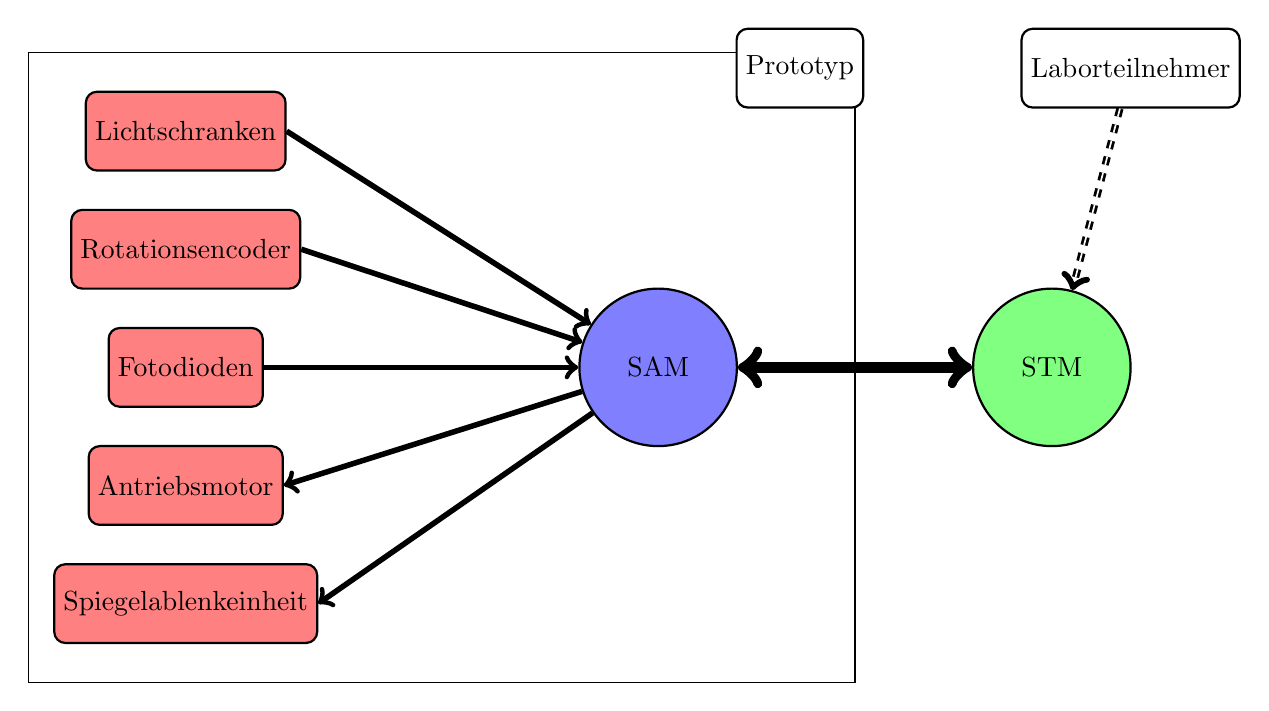
\begin{tikzpicture}[
every node/.style={draw, minimum size=1cm, thick, fill=white, rounded corners},
sam/.style={circle, minimum size=2cm, fill=blue!50},
stm/.style={circle, minimum size=2cm, fill=green!50},
sen/.style={fill=red!50}
]
\node[sam] at (6,0) (sam) {SAM};
\node[stm] at (11,0) (stm) {STM};
\node at (12,3.8) (tln) {Laborteilnehmer};
\node[sen] at (0,3) (li) {Lichtschranken};
\node[sen] at (0,1.5) (ro) {Rotationsencoder};
\node[sen] at (0,0) (fo) {Fotodioden};
\node[sen] at (0,-1.5) (an) {Antriebsmotor};
\node[sen] at (0,-3) (sp) {Spiegelablenkeinheit};

\draw[<->,line width=4pt] (sam) -- (stm);
\draw[<-,line width=2pt] (sam) -- (li.east);
\draw[<-,line width=2pt] (sam) -- (ro.east);
\draw[<-,line width=2pt] (sam) -- (fo.east);
\draw[->,line width=2pt] (sam) -- (an.east);
\draw[->,line width=2pt] (sam) -- (sp.east);
\draw[->,line width=1pt,dashed,double] (tln) -- (stm);

\draw (-2,-4) -- (-2,4) -- (8.5,4) -- (8.5,-4) -- (-2,-4);
\node at (7.8,3.8) (prot) {Prototyp};


\end{tikzpicture}

	\caption{Zusammenspiel der Komponenten}
	\label{fig:samStmSensorsAktuators}
\end{figure}

Bei diesem Prototypen existieren zwei verschiedene Controller, auf denen Software ausgeführt wird.

Der erste ist ein SAM3X8E von Atmel mit einer 32-Bit ARM Cortex-M3 Architektur.
Dieser ist auf dem Entwicklungsboard mit dem Namen "`Arduino Due"' verbaut.
Dieser Controller stellt für die Speicherung des Codes 512~KByte Flash und für Variablen 96~KByte SRAM zur Verfügung.
Auf diesem soll die Verwaltung der Hardware ablaufen.
Die Taktrate beträgt bei diesem Controller 84~MHz.

Der zweite Controller ist ein Entwicklungsboard von ST mit den Namen "`NUCLEO-F334R8"'.
Der verbaute Mikrocontroller ist ein STM32F334R8 mit einer 32-Bit ARM Cortex-M4 Architektur.
Der wesentliche Unterschied zwischen einer M3- und einer M4-Architektur liegt dabei in der zusätzlichen Gleitkommaeinheit (FPU).
Eine FPU reduziert die Dauer von Operationen mit Gleitkommazahlen erheblich.
Als Speicher stehen bei dem STM Controller 64~Kbyte Flash und 12~KByte SRAM zur Verfügung.
Die Taktfrequenz liegt bei 72~MHz.
Dieser Controller ist nur mit dem SAM3X8E verbunden und wird verwendet um den ausführbaren Code der Studierenden abzuarbeiten.
Dabei soll ein Teil der Regelung von den Studenten auf dem STM32 implementiert werden.

Der Vergleich der Controller zeigt, dass der STM32 nur eine geringfügig langsamere Taktfrequenz aufweist, dafür aber eine FPU besitzt, welche einen erheblichen Geschwindigkeitsvorteil bringt.
Der STM32 weist zusätzlich noch deutlich weniger Speicher auf, dies ist jedoch für die vorgesehene Aufgabe keine Einschränkung.
Zusammenfassend kann behauptet werden, wenn die Regelung neben den zusätzlichen Aufgaben auf dem SAM3x8E lauffähig ist, sollte die Implementierung auf dem STM32 auch kein Problem darstellen.

Um die Zusammenhänge der Komponenten deutlich zu machen, wurden die Controller und ihre Verknüpfungen in Abbildung~\ref{fig:samStmSensorsAktuators} grafisch dargestellt.
Der SAM wird als Controller zur Verwaltung der Hardware und als Schnittstelle zu den Studenten verwendet.
Der STM32 wird von den Studenten verwendet und ist nur mit dem SAM verbunden.
Im Folgenden wird vor allem der Code für den SAM erläutert.
Dieser enthält neben der Verwaltung der Hardware auch eine Musterlösung und somit den Teil, welcher im Labor auf den zweiten Controller ausgeführt wird.
Dadurch ist die gesamte Logik, zumindest für diesen Controller, implementiert.
Somit werden Ausschnitte aus dem Code in der für den SAM Controller üblichen Notation dargestellt.
Diese Notation umfasst die gebräuchlichen Typen und Befehle, welche für Arduino beziehungsweise für AVR Mikrocontroller üblich sind.
Dazu zählen auch die Integer-Typen, wie $uint16\_t$, welche in der avr-libc definiert sind.
In dieser Form sind sie auf einem STM32 standardmäßig nicht definiert.


\section{Schrittmotoren}

\subsection{Ablauf}
\label{chap:software:schrittmotoren:ablauf}
Für die Schrittmotoren wird in diesem Prototypen ein Halbschrittbetrieb verwendet.
Eine noch feinere Unterteilung ist, wie in Kapitel~\ref{chap:elektronik:mikroschrittbetrieb} erwähnt, nur begrenzt sinnvoll.
Wie bereits erläutert, können die Schrittmotoren als FSM dargestellt und behandelt werden.
Die FSM für den Halbschrittbetrieb ist in Abbildung~\ref{fig:fsmStepperHalbschritt} dargestellt.

Eine elegante Variante dies zu implementieren ist mittels eines Arrays.
Dazu wird zuerst die FSM als Array dargestellt.

\begin{minipage}{\textwidth}
\begin{lstlisting}
const uint8_t fsm[stateCnt][pinCnt] = {
	{ 1,0, 0,0 },
	{ 1,0, 1,0 },
	{ 0,0, 1,0 },
	{ 0,1, 1,0 },
	{ 0,1, 0,0 },
	{ 0,1, 0,1 },
	{ 0,0, 0,1 },
	{ 1,0, 0,1 }
};
\end{lstlisting}
\end{minipage}


Dabei stellen die beiden Pärchen des Arrays je eine Spule des Motors dar.
Vereinfacht erklärt symbolisiert eine Zahl die normierte Spannung an einem Anschluss der Spule.
Somit steht 1,0 für einen Strom in Bezugsrichtung, 0,1 für einen Strom gegen die Bezugsrichtung und 0,0 oder 1,1 für eine stromfreie Spule.
1,1 sollte jedoch nicht verwendet werden, da dies bei unipolar beschalteten Motoren zu hohen Verlusten führt.

Nun muss von einer Timer-Interrupt-Routine die aktuelle Schrittposition auf die Ausgänge des Mikrocontrollers übernommen werden.
Die Timer-Interrupt-Routine wird so eingestellt, dass sie periodisch mit der maximal erlaubten Schrittgeschwindigkeit aufgerufen wird.
Dies kann mit folgendem Code erreicht werden:

\begin{minipage}{\textwidth}
\begin{lstlisting}
int8_t state = position % stateCnt;
for (uint8_t i = 0; i < pinCnt; i++) {
	digitalWrite(pins[i], fsm[state][i]);
}
\end{lstlisting}
\end{minipage}

Dadurch ergibt sich eine asynchrone Ansteuerung der Schrittmotoren, welche unabhängig von der Geschwindigkeit des Hauptprogramms, die Motoren im richtigen Zeitpunkt ansteuert.
Dies ist deshalb besonders wichtig, da eine zu schnelle oder unregelmäßige Ansteuerung einen Schrittverlust bedeuten kann.

Vollständigkeitshalber sei hier noch erwähnt, dass der Code für einen Mikroschrittbetrieb zwar als FSM darstellbar ist, dies aber nicht zweckmäßig ist.
Eleganter ist es, mit Sinus und Kosinus zu arbeiten.
Da in diesem Fall der Mikroschrittbetrieb ohnehin nicht benötigt wird und die Berechnung von Gleitkommazahlen ohne FPU zeitaufwendig ist, wird bei dem Prototypen diese Methode nicht verwendet.

\subsection{Timing}

\begin{figure} \centering
	\includegraphics[width=0.49\textwidth]{img/PicturesPlots/Timing/StepperLaserPositioner/COPY/CONVERT/SCRN0154_Cutted.jpg}
	\caption{Dauer der Interrupts für Schrittmotoren.}
	\label{fig:interruptStepper}
\end{figure}

Für den Code, welcher in Interrupts ausgeführt wird, ist es von besonderer Bedeutung eine schnelle Verarbeitung zu erzielen.
Wenn in einem Interrupt viel Zeit benötigt wird, können dadurch andere Interrupts am Ausführen gehindert werden.
Dies ist unter allen Umständen zu vermeiden.

Die Frequenz, mit welcher der Interrupt aufgerufen wird, ist fest vorgegeben durch die Schrittgeschwindigkeit.
Der einzige Weg, den Tastgrad der Ausführungszeiten zu variieren ist somit die Rechenzeit.
Das bedeutet, dass die benötigte Rechenzeit kurz genug sein muss, um den restlichen Code nicht zu beeinflussen.

Um diese Anforderung zu überprüfen, sind in Abbildung~\ref{fig:interruptStepper} die Zeiten aufgenommen, in denen die Interrupt-Routine aktiv war.
Dabei ist der gemessene Wert auf 3,3~V wenn der Interrupt aktiv ist und 0~V wenn er nicht aktiv ist.
Der gemessene Tastgrad beträgt 1,6~\%.
Das bedeutet, dass der Interrupt nur 1,6~\% der gesamten Rechenzeit in Anspruch nimmt.
Dieser Wert ist gut vertretbar und es kann angenommen werden, dass der restliche Code unbeeinflusst abgearbeitet werden kann.



\section{Quadratur Encoder}	
Die Implementierung des Quadratur Encoders funktioniert ähnlich wie die Implementierung der Schrittmotoren.
Auch hier muss der bereits in Kapitel~\ref{chap:aufbau:aufbauInkrementalgeberFSM} betrachtete Automat implementiert werden.
Dieser kann wieder in einem Array dargestellt werden.
Hier werden jedoch nicht die Zustände als Werte der Felder verwendet, sondern die Schrittweite.
Die Indizes des Arrays stellen dabei die Zustände dar.

\begin{minipage}{\textwidth}
\begin{lstlisting}
const int8_t encoderFsm[4][4] = {
	{ 0, 1,-1, 0},
	{-1, 0, 0, 1},
	{ 1, 0, 0,-1},
	{ 0,-1, 1, 0}
};
\end{lstlisting}
\end{minipage}

Dabei hat die erste Ziffer des Zustandes die Wertigkeit 2 und die zweite Ziffer die Wertigkeit 1.
Die Zustandsnamen stellen sozusagen den Binärcode der Indizes dar.
Wird nun von dem Zustand 10 auf den Zustand 11 gewechselt, werden die Indizes 2 und 3 abgefragt und das Ergebnis ist die Schrittweite -1.

Eine wichtige Eigenschaft dieser Matrix ist, dass sie schiefsymmetrisch ist.
Das bedeutet, dass die transponierte Matrix negativ ist.
Somit liefert eine Umkehrung der Reihenfolge der Zustände ein negiertes Ergebnis.
Ein ungültiger Übergang, so wie Übergänge von einem Zustand auf sich selbst, liefert in dieser Variante 0.
Als Beispiel kann der Übergang von 01 auf 10 mit den Indizes 1 und 2 betrachtet werden.

Da jedoch Eingangsdaten und nicht Ausgangsdaten behandelt werden, funktioniert hier die Implementierung anders als die Implementierung des Schrittmotors in Kapitel~\ref{chap:software:schrittmotoren:ablauf}.
Zuerst werden die Eingangsdaten benötigt, welche mit $ina$ und $inb$ gekennzeichnet sind.
Zusätzlich ist auch der letzte Zustand von Bedeutung.
Auch dieser wird mit den zugehörigen Eingangsdaten dargestellt, welche mit $lasta$ und $lastb$ benannt sind.
Der nötige Code, um die Position zu berechnen, kann folgendermaßen geschrieben werden.

\begin{minipage}{\textwidth}
\begin{lstlisting}
pos += encoderFsm[(ina << 1) + inb][(lasta << 1) + lastb];
\end{lstlisting}
\end{minipage}

Die Erkennung der großen Marke ist mit den nun berechneten Werten trivial.
Wie in Kapitel~\ref{chap:aufbau:bigMark} bereits erläutert wurde, müssen dazu nur einzelne Schritte detektiert werden, welche ein anderes Vorzeichen aufweisen.
Auch eine Fehlerdetektion ist möglich, wenn in der Matrix spezielle Werte für einen Fehler eingetragen werden.
Ein Fehler entsteht, wenn ein Interrupt am Ausführen gehindert wird.
Dies passiert bei einer zu hohen Drehgeschwindigkeit.
Der hier präsentierte Code wird im optimalen Fall direkt von der Interrupt-Service-Routine (ISR) aufgerufen, welche für die verwendeten Eingangs-Pins zuständig und auf Pegelwechsel programmiert ist.


\section{Auswertung der Fotodioden}

\subsection{Ablauf}

Genau wie bei Schrittmotoren, ist es auch bei der Auswertung der Fotodioden sinnvoll, Interrupts zu verwenden.
Für diesen Prototypen wurde die in Kapitel~\ref{chap:elektronik:auswertung} erläuterte Methodik verwendet.

% Beschreibung der Messung
Das Messen findet in zwei verschiedenen Methoden statt.
Bei der ersten wird zuerst der Wert ermittelt, welchen die Fotodioden bei ausgeschalteten Laser zurückgeben.
Dieser Wert kann nun aufgrund der Linearität in der zweiten Methode dazu verwendet werden, langsame Störungen, wie das Tageslicht, durch Subtraktion zu eliminieren.

Diese beiden Methoden müssen abwechselnd mit Pausen dazwischen ausgeführt werden.
Am besten wird dazu ein Interrupt verwendet.
Dazu muss die Periodendauer des Interrupts bei jeder Abarbeitung umgeschaltet werden.
Die Zeiten werden im folgenden als Messzeit und Wartezeit bezeichnet
Die Messzeit ist jene, welche zwischen den beiden Methoden verstreicht.
Die Wartezeit ist die Zeit, welche zwischen der zweiten Methode und der ersten der nächsten Messung verstreicht.


\subsection{Timing}
% Tastgrad von Codeausführung
Da auch bei den Interrupts für die Fotodioden nicht zu viel Zeit verschwendet werden darf, ist besonders die Einstellung der Messfrequenz wichtig.
Bei den Schrittmotoren war die Messfrequenz gegeben, anders ist dies bei der Auswertung der Fotodioden.
Hier kann die Ausführungszeit für jede der beiden Unterfunktionen als konstant angenommen werden.
Um nun den Tastgrad auf einen vertretbaren Wert zu bringen, darf die Summe von Messzeit und Wartezeit zwischen den Messungen nicht zu niedrig liegen.
Somit muss die Messfrequenz so gewählt werden, dass ein ungestörter Programmablauf der anderen Programmteile gewährleistet werden kann.
Die Messfrequenz muss aber ausreichend hoch sein, um die Regelung nicht negativ zu beeinflussen.
Für diesen Prototypen wurde eine Messfrequenz von 200~Hz empirisch ermittelt.

% Mindestzeitdauern
Der einzige Parameter, welcher nach den bisherigen Festlegungen noch gewählt werden kann, ist die Aufteilung in Messzeit und Wartezeit.
Die Zeitdauern, welche für diese Wartezeiten mindestens eingehalten werden müssen, wurden bereits im Kapitel~\ref{chap:elektronik:transienteVorgaenge} ausgemessen.
Um eine gültige Messung zu gewährleisten, dürfen diese Zeiten auf keinen Fall unterschritten werden.

% Wahrgenommene Intensität
Solange die notwendigen Mindestzeiten eingehalten werden, verändert sich dadurch auch die Qualität der Messung nicht.
Das Verhältnis dieser Werte gibt jedoch die, von menschliche Auge wahrgenommene, Helligkeit des Laserpunktes an.
Ist die Messzeit auf den minimal erlaubten Wert eingestellt, ist der Laserpunkt unter Tageslicht kaum mehr wahrnehmbar.
Bei einer minimalen Wartezeit ergibt sich die maximale Helligkeit des Lasers.
Somit kann als Nebeneffekt dieser Regelung die gewünschte Helligkeit eingestellt werden.
Das Timing der Interrupts ist auch in diesem Fall wieder von besonderem Interesse und wird zur Überprüfung in Abbildung~\ref{fig:interruptFotodioden} dargestellt.
Der Tastgrad ist mit 8,41~\% höher als bei den Schrittmotoren aber immer noch vertretbar.
In dieser Abbildung ist auch ersichtlich, dass die Methode mit unterschiedlichen Wartezeiten aufgerufen wird.
Für diese Aufnahme wurde der Laser auf eine geringe Leuchtkraft eingestellt.
Zwischen zwei nahen Peaks ist also der Zeitraum in denen der Laser leuchtet.

\begin{figure} \centering
	\includegraphics[width=0.49\textwidth]{img/PicturesPlots/Timing/DiodesLaser/COPY/CONVERT/SCRN0160_Cutted.jpg}
	\caption{Timing der Interrupts für die Auswertung der Fotodioden.}
	\label{fig:interruptFotodioden}
\end{figure}


\section{Implementierung einer Regelung}

\subsection{Charakteristik einer Fotodiode}

\begin{figure} \centering
	\input{img/tikz/FotodiodesMeshPlotSingle}
	\caption{Ausgabewerte einer Fotodiode mit und ohne Störeinflüsse, welche im normalen Betrieb auftreten.}
	\label{img:FotodiodesSingle}
\end{figure}

Eine wichtige Grundlage beim Aufbau einer Regelung sind die zur Verfügung stehenden Informationen.
Um sich ein Bild von den möglichen Eingangsdaten zu machen, wurde mit dem Laserstrahl im Halbschrittbetrieb jeder mögliche Punkt auf den Fotodioden abgetastet.
Die Referenzspannung des ADC hat bei der Messung $3.3~V$ betragen und es wurde mit 10~Bit Auflösung gemessen.
Somit entspricht ein digitaler Wert von 1 einer Spannung von $3,22~mV$

Die Daten einer einzelnen Fotodiode wurden in Abbildung~\ref{img:FotodiodesSingle} dargestellt.
Die Grafik gibt dabei detailliert die Ausgangswerte, in Abhängigkeit zu der Schrittposition der beiden Schrittmotoren, an.
Um dabei die Übersichtlichkeit zu erhalten, wurden nur Datenpunkte angegeben, welche einen Wert von mindestens 5 aufweisen, dies entspricht $16,1~mV$.

Eine wichtige Anmerkung ist, dass die rechte Grafik auf einer Messung unter optimalen Bedingungen basiert.
Dabei wurde versucht die Fremdlichtintensität auf ein Minimum zu reduzieren.
Weiteres wurde für einen Aufnahmepunkt über 100 Messungen gemittelt.
Um eine Vorstellung davon zu bekommen, wie diese Einflüsse die Messung beeinflussen können, wurde zum Vergleich das linke Bild unter normalen Bedingungen aufgenommen.
Dabei ist deutlich sichtbar, dass die Werte gewissen Schwankungen unterliegen, die Qualität jedoch ausreichend ist, um damit eine Regelung zu implementieren.


\subsection{Charakteristik aller Fotodioden}

\begin{figure} \centering
	\begin{tikzpicture}[scale=1]
\begin{axis}[surf, z buffer=sort, opacity=0.5, restrict expr to domain={z >= 5}{1:1},xlabel=x,ylabel=y]
\addplot3 [color=red, opacity=1] table[x index=0, y index=1, z index=2, col sep=tab] {img/DiodePositionPlot/DiodePositionPlot04.txt};
\addplot3 [color=blue] table[x index=0, y index=1, z index=3, col sep=tab] {img/DiodePositionPlot/DiodePositionPlot04.txt};
\addplot3 [color=green] table[x index=0, y index=1, z index=4, col sep=tab] {img/DiodePositionPlot/DiodePositionPlot04.txt};
\addplot3 [color=orange, opacity=0.4] table[x index=0, y index=1, z index=5, col sep=tab] {img/DiodePositionPlot/DiodePositionPlot04.txt};
\end{axis}
\end{tikzpicture}
	\caption{Ausgabewerte der Fotodioden in einer gemeinsamen Grafik.}
	\label{img:FotodiodesBig}
\end{figure}

Abbildung~\ref{img:FotodiodesSingle} zeigt neben den bereits diskutierten Eigenschaften auch, dass die Fotodiode bei direkter Bestrahlung sättigt.
Dies ist für eine Regelung durchaus ein Problem und könnte behoben werden, indem der, in Kapitel~\ref{chap:elektronik:tia} besprochene Widerstand, durch einen Kleineren ersetzt wird.
Dadurch verringert sich jedoch auch die Empfindlichkeit am Rand des Messbereiches.

Wenn nun alle vier Fotodioden in ein Bild eingearbeitet werden, sieht man, dass sich die Sättigungsbereiche der Dioden kaum überlappen.
Dies wird in Abbildung~\ref{img:FotodiodesBig} dargestellt.
Selbst wenn man sich nun auf einen Punkt befindet, bei welchem zwei Dioden sättigen, so befindet man sich bereits im Messbereich der anderen beiden Dioden.
Dadurch kann im gemeinsamen Messbereich der Dioden, an den meisten Positionen der Standort bestimmt werden.


\subsection{Entwurf eines Dreipunktreglers}

%Anmerkungen zu Grafiken
Mit den bereits diskutierten Werten werden nun zwei Regler entworfen.
Ein Regler ist zuständig für den Schrittmotor, welcher den Laser horizontal ablenkt, der andere regelt die vertikale Ablenkung.
Um die Diagramme vergleichbar zu machen, zeigen sie in diesem Abschnitt immer den Regler, welcher die lange Seite der Dioden regelt.
Diese Achse wird als x Achse bezeichnen.

%Erklärung zweier Regler
Bei dem Entwurf des Reglers könnte im Folgenden berücksichtigt werden, dass die Fotodioden rechteckig sind.
Würde diese Information jedoch die Regelparameter mitbestimmen, so müsste im folgenden für jede Achse ein Regler mit verschiedenen Parametern verwendet werden.
Das soll hier für die erste Betrachtung jedoch vermieden werden.
Da nun beide Regler äquivalent zueinander sind, ist es ausreichend einen zu entwerfen.

%Einfache Verknüpfung der Daten
Das Ergebnis dieses Entwurfes soll eine Entscheidungsstrategie sein, welche entscheidet, ob der Motor in eine Bezugsrichtung drehen, gegen die Bezugsrichtung drehen oder still stehen soll.
Dafür gibt es verschiedene Strategien die gemessenen Rohdaten aufzubereiten.
So könnte zuerst die Position des Laserpunktes ermittelt werden, um mit dieser Information die Regelung durchzuführen.
Da die Position aber nichtlinear von den Eingangsdaten abhängig ist, ist es einfacher, direkt mit den Eingangsdaten der Dioden zu arbeiten.

\begin{figure} \centering
	\begin{comment}
\begin{tikzpicture}[scale=0.92]
\begin{axis}[xlabel=x,ylabel=y]
\addplot3 [surf, mesh/ordering=y varies, restrict expr to domain={z <= -4 || z >= 4 || (x > 15 && x < 25 && y > 11 && y < 28)}{1:1}] table[x index=0, y index=1, z expr={(\thisrowno{2}-\thisrowno{3})+(\thisrowno{4}-\thisrowno{5})}, col sep=tab] {img/DiodePositionPlot/DiodePositionPlot03.txt};
\end{axis}
\end{tikzpicture}
\begin{tikzpicture}[scale=0.92]
\begin{axis}[xlabel=x,ylabel=y]
\addplot3 [surf, mesh/ordering=y varies, restrict expr to domain={z <= -100 || z >= 100}{1:1}] table[x index=0, y index=1, z expr={(\thisrowno{2}-\thisrowno{3})+(\thisrowno{4}-\thisrowno{5})}, col sep=tab] {img/DiodePositionPlot/DiodePositionPlot03.txt};
\end{axis}
\end{tikzpicture}
\end{comment}
\begin{tikzpicture}[scale=0.92]
\begin{axis}[xlabel=x,ylabel=y]
\addplot3 [surf, mesh/ordering=y varies, restrict expr to domain={z <= -4 || z >= 4 || (x > 15 && x < 25 && y > 11 && y < 28)}{1:1}] table[x index=0, y index=1, z expr={(\thisrowno{2}-\thisrowno{3})+(\thisrowno{4}-\thisrowno{5})}, col sep=tab] {img/DiodePositionPlot/DiodePositionPlot03.txt};
\end{axis}
\end{tikzpicture}
\begin{tikzpicture}[scale=0.92]
\begin{axis}[xlabel=x,ylabel=y]
\addplot3 [surf, mesh/ordering=y varies, restrict expr to domain={z <= -100 || z >= 100}{1:1}] table[x index=0, y index=1, z expr={(\thisrowno{2}-\thisrowno{3})+(\thisrowno{4}-\thisrowno{5})}, col sep=tab] {img/DiodePositionPlot/DiodePositionPlot03.txt};
\end{axis}
\end{tikzpicture}
	\caption{Dreipunktregler basierend auf addierten Messwerten.}
	\label{img:dreipunktreglerAdd}
\end{figure}

Ein erster Ansatz für die Auswertung der Daten ist, die Werte auf der y Achse zu summieren und auf der x Achse zu subtrahieren.
Diese Verknüpfung der Eingangsdaten ist in Abbildung~\ref{img:dreipunktreglerAdd} im linken Bild dargestellt.
Mit den so gewonnenen Daten kann nun ein Dreipunktregler gespeist werden, welcher mit zwei Schaltschwellen entscheidet, wie der Motor angesteuert werden sollen.
Die dabei entstehende Schaltcharakteristik ist in Abbildung~\ref{img:dreipunktreglerAdd} im rechten Bild dargestellt.
Dabei wurden nur jene Bereiche gezeichnet, welche über oder unter möglichen Schwellwerten liegen.
Anders formuliert sind die Punkte des rechten Bildes die Teilmenge der Punkte des linken Bildes, bei der eine Interaktion des Motors erforderlich ist.

\begin{figure} \centering
	\input{img/tikz/FotodiodesMeshPlotMax}
	\caption{Dreipunktregler basierend auf Maximum Werte.}
	\label{img:dreipunktreglerMax}
\end{figure}

%Max Min Verknüpfung
Eine alternative Verknüpfung ist, die y Achse nicht zu summieren, sondern den Maximalwert zu verwenden.
Dadurch können Überhöhungen, welche beim Übergang von einer Fotodiode auf eine andere entstehen, vermieden werden.
Die Eingangsdaten und der Schaltbereich dieser Variante ist in Abbildung~\ref{img:dreipunktreglerMax} dargestellt.
Dabei sind die Unterschiede zur ersten Variante gut erkennbar.
Diese Unterschiede befinden sich hauptsächlich bei den Grenzbereichen der Fotodioden.


\subsection{Implementierung eines Dreipunktreglers}
Im folgenden wird die Implementierung des bereits besprochenen Dreipunktreglers gezeigt.
Dabei wird die erste Variante erläutert, bei der die Eingangswerte additiv verknüpft werden.

%Abarbeitungszyklus
Es ist wichtig, dass der Regler mit einer konstanten Frequenz periodisch aufgerufen wird.
Um eine konstante Frequenz zu gewährleisten, könnte der Regler mit einem Timer-Interrupt ausgeführt werden.
Da der Regler allerdings viele Gleitkommaoperationen benötigt und deshalb eine lange Verarbeitungszeit benötigt wird, ist dies nicht zu empfehlen.
Stattdessen wird der Regler in der Hauptschleife abgearbeitet und es wird versucht die anderen Aufgaben in Interrupts zu verlagern.
Um dabei eine konstante Abtastfrequenz zu erhalten, wird nach jedem Zyklus solange gewartet, bis der reziproke Wert der Update-Frequenz erreicht ist.

%Erklärung des Reglers
Diese Implementierung beinhaltet drei Teilaufgaben.
Die erste ist das Errechnen und Mitteln des Wertes für den Dreipunktregler.
Zur Mittlung wird ein Infinity Impulse Response (IIR) Tiefpassfilter erster Ordnung verwendet.
Der Vorteil dieses IIR Filter ist seine einfache Implementierung.
Dies kann mit folgendem Code erreicht werden.

\begin{minipage}{\textwidth}
\begin{lstlisting}
horizontal = diodeLU + diodeLD - diodeRU - diodeRD;
vertical = diodeLU + diodeRU - diodeLD - diodeRD;
lowHor = (lowHor*filterParam + horizontal) / (filterParam + 1);
lowVer = (lowVer*filterParam + vertical) / (filterParam + 1);
\end{lstlisting}
\end{minipage}

Eine schnellere und präzisere Reaktion des Reglers kann dadurch erreicht werden, dass der Filter häufiger ausgeführt wird als der Regler.
Dies sorgt für eine genauere Messung und reduziert das Rauschen und sonstige unkorrelierte Messfehler.

Die zweite Teilaufgabe ist die Berücksichtigung der Drehung der Encoderscheibe.
Dazu wird, mit dem vom Drehgeber generierten Winkel, das Koordinatensystem der Fotodioden in das der Spiegelablenkeinheit umgerechnet.
Dies kann, da die Drehung nur um die z Achse verläuft, mit einer Multiplikation mit Sinus und Kosinus erfolgen.

\begin{minipage}{\textwidth}
	\begin{lstlisting}
	double h = cos(encoderAngle);
	double v = sin(encoderAngle);
	\end{lstlisting}
\end{minipage}

Die letzte Aufgabe besteht darin, zu entscheiden ob, eine der Schaltschwellen erreicht wurde.
Wenn dies der Fall ist, kann ein Koordinaten transformierter Schritt ausgeführt werden.

\begin{minipage}{\textwidth}
\begin{lstlisting}
if (lowVer > triggerLevel) {
	stepperPosV += cosV;
	stepperPosH -= sinV;
} else if (lowVer < -triggerLevel) {
	stepperPosV -= cosV;
	stepperPosH += sinV;
}
if (lowHor > triggerLevel) {
	stepperPosH += cosV;
	stepperPosV += sinV;
} else if (lowHor < -triggerLevel) {
	stepperPosH -= cosV;
	stepperPosV -= sinV;
}
\end{lstlisting}
\end{minipage}

Hier ist es auch möglich, nicht nur einen Schritt sondern mehrere zu machen.
Ein Schritt bezeichnet dabei die kleinste verwendete Unterteilung.
Bei dem Prototypen ist dies ein Halbschritt für den Motor.

Dabei sind zwei Punkte zu beachten, damit der Regler gut funktionieren kann.
Zum ersten müssen die Schritte gerundet werden, bevor sie dem Schrittmotor als Eingangssignal gegeben werden.
Dies ist nachvollziehbar, da immer nur ein vollständiger Schritt ausgeführt werden kann, wenn nicht eine weitere Schrittteilung vorgenommen wird.

Der zweite Punkt ist, dass nicht mehr Schritte von der Regelung generiert werden dürfen, als der Motor wirklich umsetzen kann.
Dies ist für die Regelung von großer Bedeutung, da diese dadurch instabil werden kann, wenn die Motoren asynchron angesteuert werden.
Hat der Regler eine höhere Abtastrate hat als die Schrittfrequenz der Motoren, dann generiert der Regler Schritte ohne dass die Motoren die letzte Position überhaupt erreicht haben.
Erreicht der Motor danach die Soll-Position, generiert der Regler keinen Schritt mehr, die Motoren haben aber noch nicht abgearbeitete Schritte.
Dies führt zu einem Überschwingen oder zu einem instabilen Regler.
